% !TeX program = pdflatex
% Parte III de la serie godsil-gutman-lean (edición en español).
% Caminos que olvidan los ciclos — una biyección verificada por máquina entre los caminos
% tipo árbol de un grafo y los caminos del árbol de caminos de Godsil, en Lean 4.
% Compilar: pdflatex path-tree-walks-lean-es.tex  (dos veces, para las referencias)

\documentclass[11pt]{article}
\usepackage[T1]{fontenc}
\usepackage{lmodern}
\usepackage[spanish,es-noquoting]{babel}
\usepackage{amsmath,amssymb,amsthm,booktabs,graphicx,hyperref}
\usepackage{xurl}
\usepackage[table]{xcolor}
\definecolor{ggteal}{HTML}{1B6F8C}
\definecolor{ggband}{HTML}{DCE7EB}
\definecolor{ggamber}{HTML}{E08A1E}
\usepackage[margin=1in]{geometry}
\usepackage{microtype}
\usepackage[most]{tcolorbox}
\usepackage{tikz}
\usetikzlibrary{arrows.meta,positioning}
\setlength{\emergencystretch}{2em}
\graphicspath{{figures/}}
\newtheorem{theorem}{Teorema}
\newtheorem{lemma}{Lema}
\newtheorem{definition}{Definici\'on}
\newcommand{\lean}[1]{\texttt{#1}}
\newcommand{\R}{\mathbb{R}}
\newcommand{\N}{\mathbb{N}}
\DeclareMathOperator{\tr}{tr}
\hypersetup{colorlinks=true,linkcolor=ggteal,citecolor=ggteal,urlcolor=ggteal}
\newtcbox{\keybox}{on line,boxrule=0.9pt,colframe=ggteal,colback=ggband!40,
  arc=3pt,left=8pt,right=8pt,top=5pt,bottom=5pt}
\newcommand{\keyeq}[1]{\begin{center}\keybox{$\displaystyle #1$}\end{center}}

\title{\bf Caminos que olvidan los ciclos\\[4pt]
  \large\normalfont Una biyecci\'on verificada por m\'aquina entre los caminos tipo \'arbol de un grafo
  y los caminos del \'arbol de caminos de Godsil, en Lean~4}
\author{Carles Mar\'in\thanks{Formalizado con asistencia de IA (Claude, Anthropic); la matem\'atica y
todas las afirmaciones son responsabilidad del autor. La metodolog\'ia se discute en la
Secci\'on~\ref{sec:implications}.}\\[3pt]
  \normalsize Investigador independiente\\
  \normalsize \texttt{karlesmarin@gmail.com}}
\date{Junio de 2026}

\begin{document}
\maketitle

\begin{abstract}
Esta es la tercera pieza de una serie que construye, en Lean~4 / Mathlib, los dos lados de la
f\'ormula de la traza de emparejamientos/Ihara. En \emph{Desplegar un grafo en un \'arbol}~\cite{PartII}
us\'e el \emph{\'arbol de caminos} $T(G,v)$ de Godsil para demostrar que el polinomio de
emparejamientos de un grafo tiene todas sus ra\'ices reales: el \'arbol de caminos es un bosque, y un
bosque porta un espectro sim\'etrico. Aqu\'i pongo el \emph{mismo bosque} a un segundo uso. Un camino
cerrado de $G$ es \emph{tipo \'arbol} cuando nunca cierra a sabiendas un ciclo---en cada paso o avanza
a un v\'ertice nuevo o retrocede a su padre, exactamente como si caminara sobre un \'arbol. Doy una
demostraci\'on verificada por m\'aquina, \lean{sorry}-libre, de que los caminos cerrados tipo \'arbol
de $G$ con base en $v$ est\'an en biyecci\'on, que preserva la longitud, con los caminos cerrados de
$T(G,v)$ con base en su ra\'iz, realizada por la proyecci\'on hacia abajo $\pi\colon T(G,v)\to G$ que
env\'ia un camino a su extremo. Como corolario, el conteo de caminos tipo \'arbol se vuelve una suma
de potencias de la matriz de adyacencia de los \'arboles de caminos,
\[
  \mathrm{treeLikeWalkCount}(G,k)\;=\;\sum_{v}\bigl[A(T(G,v))^{k}\bigr]_{\text{ra\'iz},\text{ra\'iz}},
\]
y, como cada $T(G,v)$ es un bosque, su polinomio de emparejamientos es igual al polinomio
caracter\'istico de su matriz de adyacencia. No he hallado una formalizaci\'on previa del \'arbol de
caminos de Godsil como objeto que cuenta caminos, ni de la biyecci\'on resultante, ni del predicado
intr\'inseco ``tipo \'arbol'', en ning\'un asistente de demostraci\'on. Soy exacto sobre el l\'imite:
este art\'iculo construye la mitad \emph{combinatoria} del teorema de los momentos de Godsil
$p_k=\sum_i\theta_i^{k}=\mathrm{treeLikeWalkCount}(G,k)$. La mitad \emph{espectral} restante---la
identidad del resolvente para una entrada y el paso de Newton univariado que convierten
$[A(T)^k]_{\text{ra\'iz}}$ en un coeficiente de $\mu(G-v)/\mu(G)$---queda trazada en la
Secci\'on~\ref{sec:boundary}, no construida. Nada de esto es matem\'atica nueva; la contribuci\'on es
la formalizaci\'on, y el hecho de que el \'arbol de caminos ahora cuenta caminos en la misma
biblioteca donde ya diagonaliza un espectro.
\end{abstract}

\noindent\emph{Mapa para el lector.} Si lees una sola cosa, lee el Teorema~\ref{thm:bij}---la
biyecci\'on---y la raz\'on de una l\'inea por la que se cumple: el \'arbol de caminos es el grafo
\emph{desenrollado} hasta que los caminos se autointersecan, una \emph{inmersi\'on} de $G$ en la que un
camino se levanta a lo sumo de una forma, y se levanta exactamente cuando es tipo \'arbol. Todo lo
dem\'as es la versi\'on cuidadosa de esa frase: un lema de inyectividad local (Secci\'on~\ref{sec:inj}),
un invariante \lean{liftSeq}$\leftrightarrow$camino que hace ``tipo \'arbol'' computable y lo casa con
el levantamiento (Secci\'on~\ref{sec:inv}), y el levantamiento mismo (Secci\'on~\ref{sec:surj}). El
l\'imite honesto---la mitad espectral est\'a trazada, no construida---se enuncia tan llanamente como el
resultado.

\begin{figure}[h]
\centering
\begin{tikzpicture}[
  node distance=5mm and 9mm,
  box/.style={draw=ggteal,fill=ggband!40,rounded corners=3pt,line width=0.8pt,
    align=center,inner sep=5pt,text width=25mm,font=\small},
  mbox/.style={draw=ggamber,fill=white,rounded corners=3pt,line width=0.8pt,dashed,
    align=center,inner sep=5pt,text width=25mm,font=\small},
  arr/.style={-{Stealth[length=2.4mm]},ggteal,line width=0.9pt},
  marr/.style={-{Stealth[length=2.4mm]},ggamber,line width=0.9pt,dashed},
  lab/.style={font=\scriptsize\itshape,align=center}]
\node[box] (tl) {\textbf{caminos tipo \'arbol}\\de $G$ en $v$};
\node[box,right=of tl] (pt) {\textbf{caminos en la ra\'iz}\\de $T(G,v)$};
\node[box,right=of pt] (am) {$\bigl[A(T(G,v))^k\bigr]_{\text{ra\'iz}}$\\{\scriptsize bosque: $\mu(T)=$\,charpoly}};
\node[mbox,right=of am] (pk) {$p_k=\sum_i\theta_i^{\,k}$\\{\scriptsize momentos de $\mu(G)$}};
\draw[arr] (tl) -- node[lab,above,text=ggteal]{biyecci\'on\\(probada)} (pt);
\draw[arr] (pt) -- node[lab,above,text=ggteal]{potencia\\de matriz} (am);
\draw[marr] (am) -- node[lab,above,text=ggamber]{resolvente\,$+$\\Newton (trazado)} (pk);
\end{tikzpicture}
\caption{El recorrido del art\'iculo, y d\'onde se detiene. El conteo de caminos tipo \'arbol de $G$
iguala al conteo de caminos en la ra\'iz del \'arbol de caminos de Godsil (la biyecci\'on,
Teorema~\ref{thm:bij}), que es una potencia de la matriz de adyacencia del \'arbol
(Teorema~\ref{thm:spectral}); y cada \'arbol de caminos es un bosque, as\'i que el polinomio
caracter\'istico de esa matriz es el polinomio de emparejamientos (Teorema~\ref{thm:forest}). Las
flechas s\'olidas est\'an verificadas por m\'aquina aqu\'i; la flecha discontinua hacia los momentos
$p_k$---el resolvente de una entrada, la identidad del cociente de Godsil y el paso de Newton
univariado---est\'a trazada en la Secci\'on~\ref{sec:boundary}, no construida.}
\label{fig:spine}
\end{figure}

% ---------------------------------------------------------------
\section{Introducci\'on: un \'arbol, dos cosechas}
\label{sec:intro}

\emph{¿Cu\'ando un camino sobre un grafo no se da cuenta de que el grafo tiene ciclos---y por qu\'e
contar esos caminos olvidadizos deber\'ia recuperar los momentos de un polinomio que no es el polinomio
caracter\'istico de ninguna matriz?} Las dos mitades de esa pregunta resultan tener una sola respuesta,
un \'arbol; este art\'iculo verifica por m\'aquina la mitad combinatoria de ella.

Responderla---y explicar por qu\'e un solo artificio combinatorio zanja dos hechos sobre un grafo que
parecen no relacionados---pide que se encuentren tres hilos de historia.

\paragraph{Un polinomio con ra\'ices reales y sin matriz (1972).} Un grafo finito $G$ tiene un
polinomio de emparejamientos $\mu(G,x)=\sum_{k}(-1)^k m_k(G)\,x^{n-2k}$, donde $m_k(G)$ cuenta sus
emparejamientos de $k$ aristas~\cite{Farrell1979,LovaszPlummer}. En 1972 Heilmann y Lieb, estudiando
sistemas de mon\'omeros y d\'imeros en mec\'anica estad\'istica, demostraron que sus ra\'ices son
siempre reales~\cite{HeilmannLieb}---un enunciado sobre transiciones de fase en f\'isica, espectral en
combinatoria. Pero las ra\'ices reales son la firma de una \emph{matriz sim\'etrica}, y $\mu(G)$ no es
el polinomio caracter\'istico de ninguna matriz fija salvo que $G$ sea un bosque. As\'i que la pregunta
se afila: si no hay matriz, ¿de d\'onde salen las ra\'ices reales, y el contenido combinatorio de sus
sumas de potencias $p_k=\sum_i\theta_i^{k}$?

\paragraph{Un \'arbol, dos teoremas (1981).} La respuesta de Godsil fue un solo
artificio~\cite{Godsil1981a,Godsil1981b,GodsilBook}. Dado un v\'ertice $v$, el \emph{\'arbol de
caminos} $T(G,v)$ tiene como v\'ertices los caminos simples de $G$ que empiezan en $v$, y une un camino
a otro cuando el segundo extiende al primero por una sola arista. Es un bosque---la truncaci\'on finita
del \emph{recubrimiento universal} de $G$ desenrollado desde $v$---y de \'el Godsil sac\'o dos
conclusiones. Primero, $\mu(G)\mid\mu(T(G,v))$, y el polinomio de emparejamientos de un bosque \emph{es}
el polinomio caracter\'istico de su matriz de adyacencia, luego de ra\'ices reales; esto recupera
Heilmann--Lieb, y es lo que formaliz\'o la Parte~II de esta serie~\cite{PartII}. Segundo---el tema de
este art\'iculo---el \'arbol de caminos \emph{cuenta caminos}.

\paragraph{Caminos, recubrimientos y una f\'ormula de traza.} El recubrimiento universal es el objeto
m\'as profundo tras el \'arbol finito: el radio espectral del \'arbol infinito $(\Delta-1)$-regular es
$2\sqrt{\Delta-1}$, el borde \emph{Ramanujan}, que es tambi\'en la cota de Godsil sobre las ra\'ices de
emparejamiento, y el espectro del recubrimiento est\'a gobernado por el polinomio de
emparejamientos~\cite{AngelFriedmanHoory,Spier2025}. Del lado finito esto es una \emph{f\'ormula de
traza}: $\tr(A^k)$ cuenta \emph{todos} los caminos cerrados de $G$, mientras que $p_k$ cuenta solo los
\emph{tipo \'arbol}; por debajo de la cintura todo camino es tipo \'arbol, as\'i que ambos coinciden, y
la primera diferencia cuenta los ciclos m\'as cortos. El lado ciclo, $\tr(A^k)$ y su refinamiento de
no-retroceso, es el complemento \emph{Bass} de esta serie~\cite{Bass,Hashimoto,IharaBass}; este
art\'iculo construye la mitad combinatoria del lado \'arbol.

Un camino cerrado de $G$ es \emph{tipo \'arbol} cuando, visto paso a paso, solo avanza a un v\'ertice
nuevo o retrocede al v\'ertice del que vino: nunca atraviesa una arista de vuelta a un v\'ertice
anterior que no sea su padre, as\'i que nunca cierra a sabiendas un ciclo. (Puede, en conjunto,
atravesar las tres aristas de un tri\'angulo---siempre que cada \emph{camino} intermedio siga simple;
es justo ah\'i donde falla la definici\'on ingenua, Figura~\ref{fig:moments}.) La observaci\'on de
Godsil es que estos son precisamente los caminos que $G$ hereda de $T(G,v)$: un camino cerrado en la
ra\'iz del \'arbol de caminos, empujado hacia abajo a $G$ registrando solo el extremo actual, es un
camino cerrado tipo \'arbol en $v$, y todo camino tipo \'arbol surge as\'i, de forma \'unica
(Figura~\ref{fig:bij}). Sumando sobre $v$ y sobre los caminos de longitud $k$ se obtiene
$\mathrm{treeLikeWalkCount}(G,k)$, y el teorema de los momentos lo identifica con $p_k(G)$.

\paragraph{Por qu\'e formalizarlo.} El polinomio de emparejamientos est\'a en la intersecci\'on de tres
hilos de esta serie---ra\'ices reales (Partes~I--II~\cite{PartI,PartII}), la f\'ormula de la traza de
emparejamientos/Ihara (el complemento \emph{Bass}~\cite{Bass}) y, por el borde de banda
$2\sqrt{\Delta-1}$, los grafos de Ramanujan~\cite{MSS}. La f\'ormula de la traza tiene un lado
\emph{ciclo}, $\tr(A^k)$ contando todos los caminos cerrados, y un lado \emph{\'arbol}, $p_k$ contando
los tipo \'arbol; por debajo de la cintura coinciden, y la primera diferencia es un conteo de ciclos
cortos. Para enunciar ese puente dentro de un asistente de demostraci\'on hace falta el lado \'arbol
como objeto honesto, y el lado \'arbol es precisamente un enunciado sobre el \'arbol de caminos. La
Parte~II construy\'o el \'arbol de caminos por su espectro; este art\'iculo ense\~na al mismo objeto de
Lean a contar.

\paragraph{Qu\'e hay de nuevo aqu\'i, y qu\'e no.} La matem\'atica es de Godsil. La contribuci\'on es la
construcci\'on verificada por m\'aquina: el \'arbol de caminos como grafo que cuenta caminos, la
proyecci\'on hacia abajo como homomorfismo de grafos que es una \emph{inmersi\'on}, un predicado
decidible intr\'inseco \lean{IsTreeLike} que computa el levantamiento como una disciplina de pila, el
invariante que ata esa pila al v\'ertice actual del \'arbol de caminos, el levantamiento en la
direcci\'on sobreyectiva, y la biyecci\'on de cardinales resultante. De ninguno de ellos hall\'e una
formalizaci\'on previa en ning\'un asistente de demostraci\'on. El enunciado principal depende solo de
los tres axiomas est\'andar (\lean{propext}, \lean{Classical.choice}, \lean{Quot.sound}); no hay
\lean{sorry}.

% ---------------------------------------------------------------
\section{Los dos lados, mantenidos aparte}
\label{sec:objects}

\emph{¿Qu\'e, exactamente, estamos casando---y c\'omo evitamos que los dos lados sean el mismo objeto
con dos sombreros?} Una biyecci\'on solo dice algo cuando sus extremos se definen sin referencia uno al
otro; as\'i que fijo ambos, y solo despu\'es dejo que se encuentren. En todo lo que sigue, $G$ es un
\lean{SimpleGraph} sobre un tipo de v\'ertices $V$, y $v\in V$ es un punto base. Reutilizo el \'arbol de
caminos de la Parte~II tal cual.

\begin{definition}[\'Arbol de caminos, \lean{pathTree}]
Los v\'ertices de $T(G,v)=\lean{pathTree}\,G\,v$ son los caminos simples de $G$ que empiezan en $v$
(\lean{PathFrom}\,$v=\Sigma_{u}\,G.\mathrm{Path}\,v\,u$). Dos son adyacentes cuando uno se obtiene del
otro a\~nadiendo una sola arista al final (\lean{Grows}). La ra\'iz es el camino trivial en $v$
(\lean{pathTreeRoot}). Es un bosque: \lean{pathTree\_isAcyclic}.
\end{definition}

\begin{definition}[Proyecci\'on hacia abajo, \lean{pathTreeProj}]
$\pi\colon T(G,v)\to G$ env\'ia un camino a su extremo, $\pi\langle u,p\rangle=u$. La adyacencia en el
\'arbol de caminos significa que un camino extiende al otro por una arista, as\'i que los dos extremos
son adyacentes en $G$; por tanto $\pi$ es un homomorfismo de grafos, y $\pi(\text{ra\'iz})=v$.
\end{definition}

El predicado tipo \'arbol se define de forma intr\'inseca, sin referencia al \'arbol de caminos, para
que los dos lados de la biyecci\'on sean objetos genuinamente distintos por casar. Un camino cerrado
$w$ en $v$ se alimenta, v\'ertice a v\'ertice (su soporte salvo la primera entrada), a un
\emph{levantamiento} determinista \lean{liftSeq} que enhebra una pila---el camino simple actual desde
$v$. Para cada v\'ertice siguiente $c$: si $c$ no est\'a en la pila, lo \emph{apila} (un \textsc{avance});
si $c$ es el pen\'ultimo v\'ertice de la pila, \emph{desapila} (un \textsc{retroceso} al padre); en otro
caso el levantamiento \emph{falla}. Los dos casos son mutuamente excluyentes, as\'i que el levantamiento
es un \emph{fold}.

\begin{definition}[Tipo \'arbol, \lean{Walk.IsTreeLike}]
$w$ es \emph{tipo \'arbol} si su levantamiento, comenzado desde la pila ra\'iz $[v]$, vuelve a $[v]$:
$\lean{liftSeq}\;w.\mathrm{support}.\mathrm{tail}\;[v]=\lean{some}\,[v]$. Es decidible.
\end{definition}

Esta definici\'on es la corregida. La elecci\'on ingenua---``el soporte de aristas de $w$ es
ac\'iclico''---es \emph{falsa} para el teorema de los momentos: en $K_4$ con $k=6$ subcuenta ($276$
frente a $p_6=324$), porque un camino tipo \'arbol puede atravesar las aristas de un ciclo en conjunto.
El predicado \lean{liftSeq} se valid\'o num\'ericamente contra las sumas de potencias de emparejamiento
en $P_4,C_4,C_5,K_4$ y los grafos de Petersen y $K_{3,3}$ para $k\le8$ antes de formalizarlo
(Figura~\ref{fig:moments}).

\begin{figure}[t]
  \centering
  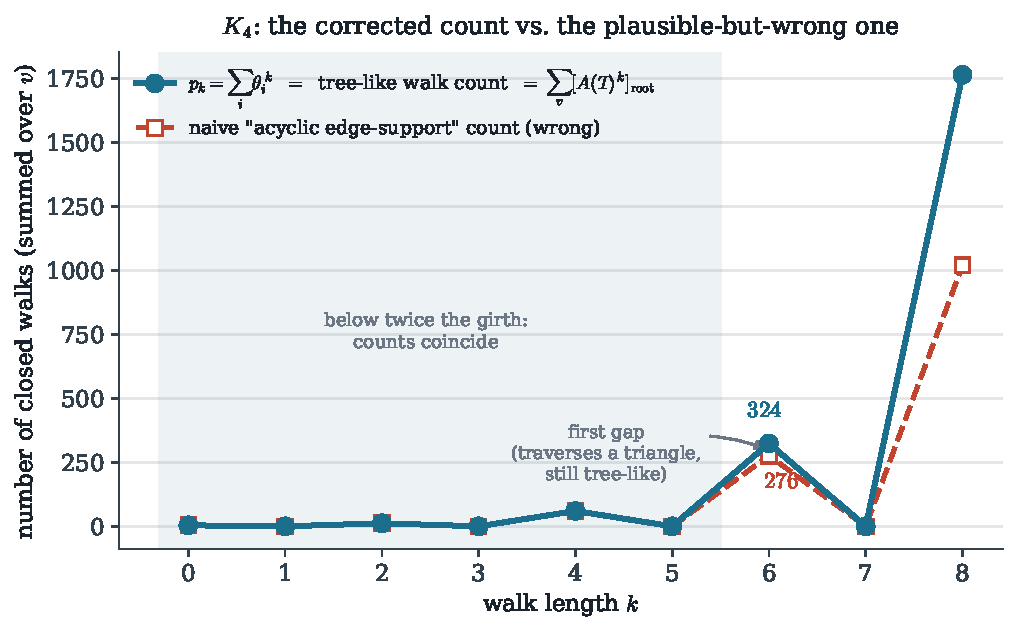
\includegraphics[width=0.82\textwidth]{pt_fig2_moments.pdf}
  \caption{Por qu\'e importa la definici\'on, en $K_4$. Las sumas de potencias de emparejamiento $p_k$
  (turquesa) coinciden con el conteo tipo \'arbol / del \'arbol de caminos para todo $k$---la biyecci\'on
  de este art\'iculo hace exacta la segunda igualdad. El conteo plausible de ``soporte de aristas
  ac\'iclico'' (rojo) concuerda hasta $k=5$ pero luego subcuenta, $276$ frente a $324$ en $k=6$, porque
  un camino tipo \'arbol puede atravesar las tres aristas de un tri\'angulo mientras cada camino
  intermedio sigue simple. Una comprobaci\'on num\'erica barata atrap\'o la definici\'on equivocada
  antes de gastar esfuerzo formal en ella.}
  \label{fig:moments}
\end{figure}

% ---------------------------------------------------------------
\section{El resultado}
\label{sec:result}

\begin{theorem}[La biyecci\'on, \lean{card\_treeLike\_eq\_pathTreeWalks}]\label{thm:bij}
Para todo grafo finito $G$, punto base $v$ y longitud $k$, la aplicaci\'on $W\mapsto W.\mathrm{map}\,\pi$
es una biyecci\'on de los caminos cerrados de longitud $k$ en la ra\'iz de $T(G,v)$ sobre los caminos
cerrados tipo \'arbol de longitud $k$ de $G$ en $v$. En particular sus cardinales coinciden:
\keyeq{\#\{\,\text{caminos tipo \'arbol de }G\text{ en }v,\ \text{longitud }k\,\}
   \;=\;\#\{\,\text{caminos en la ra\'iz de }T(G,v),\ \text{longitud }k\,\}.}
\end{theorem}

\begin{figure}[t]
  \centering
  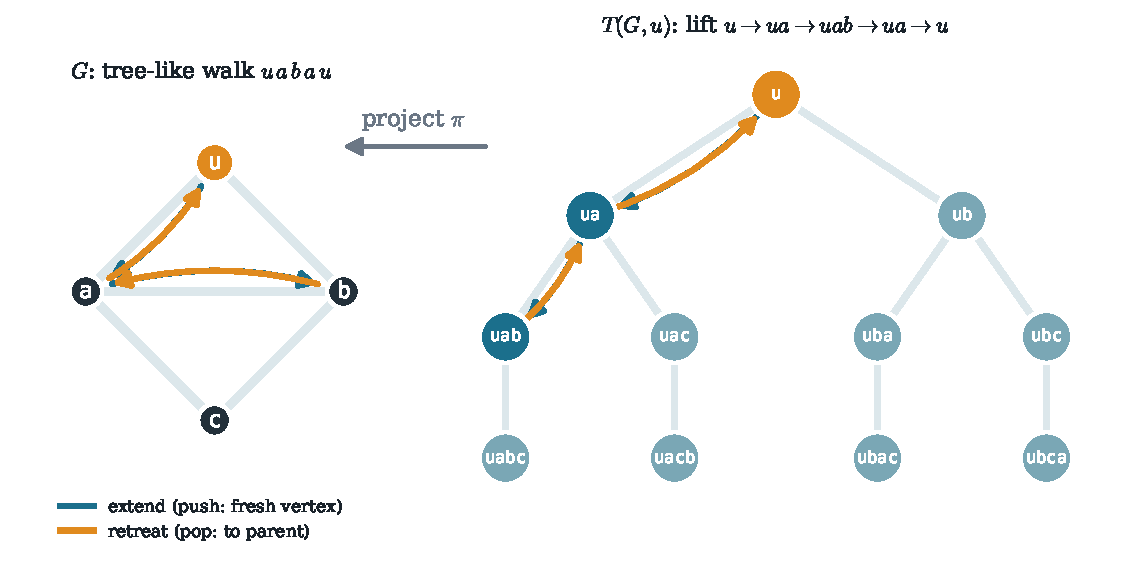
\includegraphics[width=0.96\textwidth]{pt_fig1_bijection.pdf}
  \caption{La biyecci\'on en el diamante $G=K_4-e$, ra\'iz $u$. Un camino cerrado en la ra\'iz del
  \'arbol de caminos $T(G,u)$ (derecha), $u\to ua\to uab\to ua\to u$, se proyecta bajo $\pi$ (un camino
  $\mapsto$ su extremo) a un camino cerrado tipo \'arbol de $G$ (izquierda), $u\,a\,b\,a\,u$. Cada paso
  es un \textsc{avance} (turquesa, ir a un v\'ertice nuevo / apilar) o un \textsc{retroceso} (\'ambar,
  volver al padre / desapilar). El camino de la izquierda recorre las aristas $ua,ab$ hacia afuera y las
  retraza de vuelta; el levantamiento de la derecha hace expl\'icita la historia del camino, y es el
  \'unico camino sobre ella.}
  \label{fig:bij}
\end{figure}

\emph{¿Qu\'e hace falta para fiarse de una biyecci\'on?} Una aplicaci\'on, y su promesa cumplida en dos
direcciones. La aplicaci\'on es $\pi$ le\'ida sobre caminos enteros, $W\mapsto W.\mathrm{map}\,\pi$; su
promesa son tres hechos, y las tres secciones de demostraci\'on que siguen son, en orden, exactamente
esos tres. La aplicaci\'on debe \emph{aterrizar donde debe}: un camino-\'arbol proyectado es siempre
tipo \'arbol, as\'i que $\pi$ lleva los caminos del \'arbol \emph{dentro} de los tipo \'arbol de $G$
(Lema~\ref{lem:img}, ganado en la Secci\'on~\ref{sec:inv}). Debe \emph{no olvidar nada}: dos
caminos-\'arbol no proyectan la misma sombra (Lema~\ref{lem:inj}, Secci\'on~\ref{sec:inj}). Y debe
\emph{no perder nada}: todo camino tipo \'arbol es la sombra de alg\'un camino---el levantamiento existe
(Lema~\ref{lem:surj}, Secci\'on~\ref{sec:surj}). Aterriza, inyectiva, sobreyectiva; eso es todo el
Teorema~\ref{thm:bij}, y el resto del art\'iculo son esas tres palabras hechas precisas.

\begin{lemma}[La imagen es tipo \'arbol, \lean{pathTreeProj\_map\_isTreeLike}]\label{lem:img}
La $\pi$-proyecci\'on de cualquier camino cerrado en la ra\'iz de $T(G,v)$ es tipo \'arbol.
\end{lemma}

\begin{lemma}[Inyectividad, \lean{pathTreeProj\_walk\_injective}]\label{lem:inj}
$W\mapsto W.\mathrm{map}\,\pi$ es inyectiva sobre los caminos de $T(G,v)$.
\end{lemma}

\begin{lemma}[Sobreyectividad / el levantamiento, \lean{exists\_root\_lift}]\label{lem:surj}
Todo camino cerrado tipo \'arbol de $G$ en $v$ es $W.\mathrm{map}\,\pi$ para alg\'un camino cerrado $W$
en la ra\'iz de $T(G,v)$.
\end{lemma}

\emph{Una biyecci\'on que solo renombra un conjunto finito es contabilidad---¿qu\'e compra entonces
esta?} Su valor es que los dos lados son \emph{tipos} de objeto distintos: a la izquierda, un conteo
combinatorio; a la derecha, caminos sobre un \emph{\'arbol}. Y un \'arbol tiene una matriz. As\'i que el
conteo de la derecha es una potencia de matriz, una potencia de matriz es una cantidad espectral, y el
renombrado nos ha movido, calladamente, al lado espectral, donde vive el resto del teorema de los
momentos. Dos corolarios dan el paso.

\begin{theorem}[Forma espectral, \lean{treeLikeWalkCount\_eq\_sum\_pathTree\_adjMatrix\_pow}]
\label{thm:spectral}
\[
  \mathrm{treeLikeWalkCount}(G,k)\;=\;\sum_{v\in V}\bigl[A(T(G,v))^{k}\bigr]_{\text{ra\'iz},\text{ra\'iz}}.
\]
\end{theorem}

\begin{theorem}[Puente del bosque, \lean{matchingPoly\_pathTree\_eq\_charpoly}]\label{thm:forest}
Cada \'arbol de caminos es un bosque, as\'i que su polinomio de emparejamientos es el polinomio
caracter\'istico de su matriz de adyacencia: $\mu(T(G,v))=\mathrm{charpoly}\bigl(A(T(G,v))\bigr)$.
\end{theorem}

% ---------------------------------------------------------------
\section{El \'arbol de caminos es una inmersi\'on}
\label{sec:inj}

\emph{Si el \'arbol de caminos es el grafo desenrollado, ¿qu\'e impide que un camino se desenrolle de
forma ambigua---que tenga dos levantamientos distintos?} La respuesta es local, y es todo el motor de la
inyectividad. Los vecinos de un v\'ertice $p$ del \'arbol de caminos son su \'unico padre (quitar la
\'ultima arista) y sus hijos (a\~nadir una arista cada uno). La proyecci\'on $\pi$ env\'ia el padre al
pen\'ultimo v\'ertice de $p$, que est\'a sobre $p$, y cada hijo a su extremo nuevo, que no lo est\'a; y
hijos distintos tienen extremos distintos. As\'i que $\pi$ \emph{separa} los vecinos de cada v\'ertice:
\lean{pathTreeProj\_injOn\_neighborSet}. La mitad del padre es \lean{Grows.parent\_unique} de la
Parte~II; su dual \lean{Grows.child\_unique} (una extensi\'on por una arista queda determinada por su
extremo) es nuevo aqu\'i.

\begin{figure}[t]
  \centering
  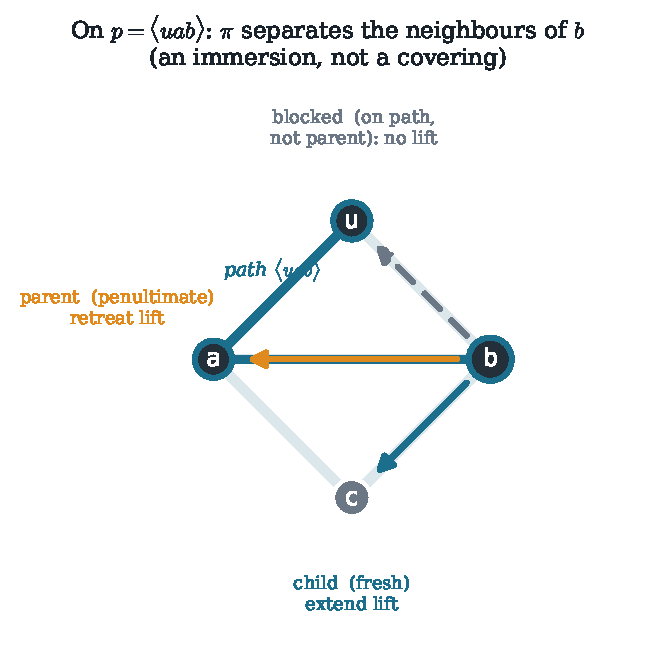
\includegraphics[width=0.62\textwidth]{pt_fig4_immersion.pdf}
  \caption{La inmersi\'on, en el v\'ertice $p=\langle uab\rangle$ del \'arbol de caminos (el camino
  $u\,a\,b$, turquesa). El paso siguiente mira los vecinos del extremo $b$, que en $G$ son $a$, $c$, $u$.
  Cada uno cae en exactamente un caso: $a$ es el pen\'ultimo de $p$ (el \emph{padre}, un retroceso), $c$
  es nuevo (un \emph{hijo}, un avance), y $u$ est\'a sobre $p$ pero no es su padre---\emph{bloqueado},
  sin levantamiento por encima de $p$. As\'i $\pi$ es inyectiva sobre los vecinos de $p$ pero no
  sobreyectiva; la direcci\'on bloqueada es por lo que el \'arbol de caminos es una inmersi\'on, y por lo
  que un camino proyectado solo puede ser tipo \'arbol.}
  \label{fig:immersion}
\end{figure}

Esta inyectividad local es exactamente la propiedad de inmersi\'on: $\pi$ es localmente inyectiva pero no
localmente sobreyectiva---un $G$-vecino del extremo de $p$ que ya est\'a sobre $p$ no tiene preimagen por
encima de $p$. Esa asimetr\'ia es toda la historia. Y es tambi\'en una vieja con otro traje: una
aplicaci\'on recubridora, en el sentido de la topolog\'ia de Poincar\'e, levanta \emph{todo} camino de
forma \'unica; una inmersi\'on solo levanta los caminos que nunca se doblan sobre s\'i mismos---y
``nunca se dobla hacia un v\'ertice que no es el padre'' es precisamente lo que significa tipo \'arbol. Un camino en $T(G,v)$ queda determinado, paso a paso,
por su $\pi$-imagen junto con su inicio, porque en cada v\'ertice el siguiente v\'ertice del \'arbol de
caminos est\'a forzado por la inyecci\'on local; una inducci\'on que imita a
\lean{Walk.map\_injective\_of\_injective} de Mathlib, con la hip\'otesis global reemplazada por la
local, da el Lema~\ref{lem:inj}.

% ---------------------------------------------------------------
\section{El invariante \texttt{liftSeq}$\leftrightarrow$camino}
\label{sec:inv}

\emph{\lean{IsTreeLike} es una disciplina de pila sobre $G$ solo---el \'arbol de caminos no aparece en
\'el---¿por qu\'e deber\'ia detectar exactamente los caminos que vienen del \'arbol?} Porque la pila
\emph{es} el v\'ertice del \'arbol disfrazado. Leer un camino como una sucesi\'on de apilados y
desapilados es el movimiento m\'as antiguo de la combinatoria enumerativa---el problema de la votaci\'on,
las palabras equilibradas de von Dyck, los n\'umeros de Catalan viven todos sobre la misma pila---y
aqu\'i es el puente, en forma de un solo invariante: al caminar $T(G,v)$, ejecutar \lean{liftSeq} sobre
el camino proyectado rastrea el v\'ertice actual del \'arbol de caminos.

\begin{lemma}[Un paso, \lean{liftSeq\_step}]
Para una arista $s\sim y$ del \'arbol de caminos y cualquier cola $M$,
$\lean{liftSeq}\,(y_1::M)\,s.\mathrm{support}=\lean{liftSeq}\,M\,y.\mathrm{support}$: un paso a un hijo
es un \textsc{apilar}, un paso al padre es un \textsc{desapilar}.
\end{lemma}

\begin{lemma}[Invariante, \lean{liftSeq\_map\_invariant}]\label{lem:inv}
Para un camino $W\colon s\to x$ del \'arbol de caminos,
$\lean{liftSeq}\,(W.\mathrm{map}\,\pi).\mathrm{support}.\mathrm{tail}\,\;s.\mathrm{support}
=\lean{some}\,x.\mathrm{support}$.
\end{lemma}

El Lema~\ref{lem:img} es el caso $s=x=\text{ra\'iz}$, cuyo soporte de camino es $[v]$. El mismo
invariante impulsa el levantamiento: es la contabilidad que, ejecutada al rev\'es, reconstruye el camino
del \'arbol de caminos a partir de un camino tipo \'arbol.

\begin{figure}[t]
  \centering
  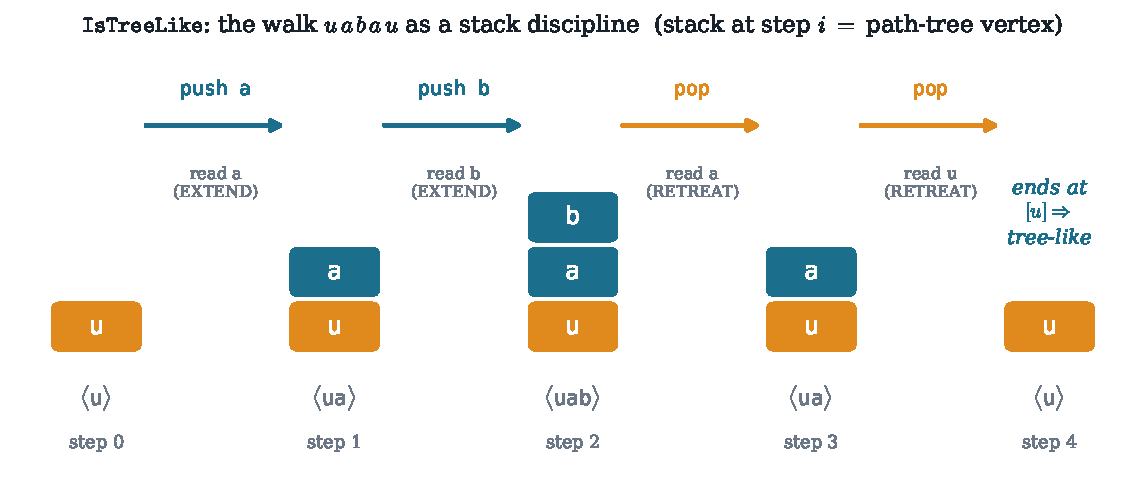
\includegraphics[width=0.97\textwidth]{pt_fig3_stack.pdf}
  \caption{\lean{IsTreeLike} como disciplina de pila---el predicado \lean{liftSeq} ejecutado sobre el
  camino $u\,a\,b\,a\,u$. La pila es el camino simple actual desde $u$; cada v\'ertice siguiente se lee y
  o se \textsc{apila} (avance, turquesa: un v\'ertice nuevo) o se \textsc{desapila} (retroceso, \'ambar:
  es el pen\'ultimo). El camino es tipo \'arbol si la pila termina de vuelta en $[u]$. La pila en el paso
  $i$ es exactamente el v\'ertice del \'arbol de caminos sobre el que se sit\'ua el levantamiento---$
  \langle u\rangle,\langle ua\rangle,\langle uab\rangle,\langle ua\rangle,\langle u\rangle$---que es el
  contenido del invariante, Lema~\ref{lem:inv}.}
  \label{fig:stack}
\end{figure}

% ---------------------------------------------------------------
\section{El levantamiento: trepar de vuelta al \'arbol}
\label{sec:surj}

\emph{Todo camino tipo \'arbol deber\'ia venir del \'arbol---pero ¿c\'omo exhibimos el camino del que
viene, cuando sus propios extremos en el \'arbol no se dan sino que se computan?} La sobreyectividad es
la \'unica direcci\'on que construye un camino en el tipo dependiente $(T(G,v)).\mathrm{Walk}$, y sus
extremos se computan, no se dan. La construcci\'on (\lean{exists\_lift}) es una recursi\'on sobre el
$G$-camino: la hip\'otesis ``\lean{liftSeq} acepta $w$ desde el v\'ertice actual'' suministra, en cada
paso, la decisi\'on \textsc{avance}/\textsc{retroceso}, as\'i que no hay rama de fallo. El v\'ertice
actual del \'arbol de caminos se lleva como la terna expl\'icita $\langle a, pp, hpp\rangle$ (extremo,
camino, prueba-de-que-es-camino), lo que esquiva las igualdades heterog\'eneas que un acumulador de tipo
$\Sigma$ forzar\'ia. Dos fricciones m\'as se manejan con el mismo truco: la recursi\'on demuestra
igualdad de \emph{soportes} (una \lean{List}~$V$, libre de tipos dependientes) en lugar de igualdad de
caminos, y \lean{Walk.support\_injective} eleva la igualdad de soportes a igualdad de caminos una vez
fijados los extremos en el corolario del camino cerrado (Lema~\ref{lem:surj}). El levantamiento vuelve a
la ra\'iz porque su soporte de camino final es $[v]$, forzando que el v\'ertice-\'arbol final sea el
camino trivial.

La biyecci\'on (Teorema~\ref{thm:bij}) es entonces \lean{Finset.card\_bij} sobre $W\mapsto
W.\mathrm{map}\,\pi$, con el Lema~\ref{lem:img} para la buena definici\'on, el Lema~\ref{lem:inj} para la
inyectividad y el Lema~\ref{lem:surj} para la sobreyectividad; las longitudes se preservan porque
$\mathrm{map}$ las preserva.

% ---------------------------------------------------------------
\section{El l\'imite: qu\'e se construye y qu\'e se traza}
\label{sec:boundary}

\emph{La biyecci\'on cuenta; el teorema de los momentos iguala ese conteo con un espectro. ¿D\'onde,
exactamente, termina el terreno verificado por m\'aquina y empieza el \'algebra trazada-pero-sin-construir?}
El teorema de los momentos de Godsil es
\keyeq{p_k(G)\;=\;\sum_i\theta_i^{k}\;=\;\mathrm{treeLikeWalkCount}(G,k).}
Este art\'iculo construye su mitad \emph{combinatoria}---todo hasta la forma espectral
(Teorema~\ref{thm:spectral}) y el puente del bosque (Teorema~\ref{thm:forest}) inclusive. La mitad
\emph{espectral} se traza aqu\'i pero no se formaliza; la enuncio llanamente para que el lector sepa
exactamente d\'onde acaba el terreno verificado por m\'aquina.

La cadena restante es \'algebra est\'andar. Para cada \'arbol de caminos $T=T(G,v)$, el resolvente de la
entrada ra\'iz--ra\'iz genera los conteos de caminos,
\[
  \sum_{k\ge0}\bigl[A(T)^k\bigr]_{\text{ra\'iz}}X^{k}
  \;=\;\frac{\mathrm{charpolyRev}\bigl(A(T)_{\widehat{\text{ra\'iz}}}\bigr)}{\mathrm{charpolyRev}(A(T))},
\]
el caso de una entrada de $\mathrm{adj}(1-XA)=\det(1-XA)\,(1-XA)^{-1}$, que esta biblioteca ya tiene en
forma matricial (\lean{smul\_resolventSeries\_eq\_adjugate}, \lean{coeff\_resolventSeries}). Lo que
\emph{a\'un no} est\'a en Mathlib, y es el \'unico lema de \'algebra lineal genuinamente nuevo que la
completaci\'on necesita, es la identidad del menor principal
$\mathrm{adj}(M)_{ii}=\det\bigl(M\!\restriction_{j\neq i}\bigr)$ sobre un tipo de \'indices finito
arbitrario (Mathlib solo tiene la expansi\'on por cofactores para \lean{Fin}). Concedi\'endolo, el puente
del bosque convierte cada $\mathrm{charpolyRev}$ en un polinomio de emparejamientos invertido; la
\lean{godsil\_identity} de la Parte~II, $\mu(G)\,\mu(T-\text{ra\'iz})=\mu(G-v)\,\mu(T)$, reescribe
el cociente como $\mu(G-v)/\mu(G)$; la ley de la derivada por borrado de v\'ertice
$\sum_v\mu(G-v)=X\,\mu'(G)$ (ya demostrada, \lean{sum\_matchingPoly\_deleteIncidenceSet}) lo suma a
$\mu'(G)/\mu(G)$; y la identidad de Newton univariada iguala esa derivada logar\'itmica con
$\sum_k p_k X^{k}$. Igualando los coeficientes de $X^k$ se cierra el teorema. El \'ultimo paso es venerable en s\'i: las
identidades de Newton, que relacionan las sumas de potencias de un polinomio con sus coeficientes, las
escribi\'o Girard en 1629 y Newton una generaci\'on m\'as tarde, y el teorema de los coeficientes de
Sachs de 1964 lee esos coeficientes en los propios subgrafos del grafo. Dos de los eslabones---el lema
del menor principal y el puente de Newton para ra\'ices univariadas---son resultados generales ausentes
de Mathlib, y ambos se guardan en la zona \texttt{MathlibPR} del repositorio en forma can\'onica, sin
grafos.

% ---------------------------------------------------------------
\section{Implicaciones y metodolog\'ia}
\label{sec:implications}

El autor fij\'o los objetivos y dirimi\'o la matem\'atica; el asistente (Claude, Anthropic) redact\'o las
demostraciones y esta prosa. Todo teorema citado aqu\'i compila \lean{sorry}-libre contra la revisi\'on
fijada de Mathlib~\cite{Mathlib} y depende solo de los tres axiomas est\'andar, lo que el lector puede
reverificar con \lean{\#print axioms}. La definici\'on ``tipo \'arbol'' corregida es en s\'i un peque\~no
dato metodol\'ogico: la lectura natural por soporte ac\'iclico es plausible, compila, y es \emph{falsa}
para el teorema al que debe servir; una comprobaci\'on num\'erica barata contra las sumas de potencias de
emparejamiento la atrap\'o antes de gastar esfuerzo formal, y la misma comprobaci\'on certifica la
definici\'on \lean{liftSeq} que la reemplaz\'o.

\paragraph{Para qu\'e sirve---y para qu\'e no.} Los objetos de aqu\'i no son ex\'oticos. El polinomio de
emparejamientos es la funci\'on de partici\'on mon\'omero--d\'imero de la mec\'anica
estad\'istica~\cite{HeilmannLieb}; los momentos de sus ra\'ices son la materia prima del m\'etodo de los
momentos para acotar autovalores; la cota que esos momentos obedecen, $2\sqrt{\Delta-1}$, es el umbral
que un grafo debe superar para ser un expansor; y el objeto espectral de al lado, el operador de
no-retroceso, fija el umbral de percolaci\'on de una red~\cite{Hashimoto,Bass}. Este art\'iculo no
a\~nade nada a eso. Solo pone una mitad del puente que esos m\'etodos cruzan---el lado \'arbol de la
f\'ormula de la traza---sobre terreno certificado, en la misma biblioteca que el lado ciclo, y deja tras
de s\'i un peque\~no objeto reutilizable, el \'arbol de caminos, que ya hizo un trabajo (un espectro
real, Parte~II) y ahora hace un segundo. Ning\'un algoritmo y ninguna red: un cimiento, y uno modesto.

La matem\'atica es de Godsil, de hace cuatro d\'ecadas. Solo la he llevado, con cuidado, a una forma que
una m\'aquina comprobar\'a: en la Parte~II el \'arbol de caminos porta un espectro real, y aqu\'i cuenta
los caminos que un grafo confunde con un \'arbol. El lado ciclo de la f\'ormula de la traza de
emparejamientos/Ihara---$\tr(A^k)$---est\'a en la misma biblioteca (el complemento \emph{Bass}~\cite{Bass});
si alg\'un d\'ia se construyera la mitad espectral de la Secci\'on~\ref{sec:boundary}, el lado \'arbol
$p_k$ se encontrar\'ia con \'el, y la f\'ormula de la traza ser\'ia una sola l\'inea verificada por
m\'aquina. Eso queda, sin disculpas, para otro d\'ia.

% ---------------------------------------------------------------
\section{Preguntas que quedan abiertas}
\label{sec:questions}

Una formalizaci\'on es tambi\'en una lista de las pr\'oximas preguntas, afiladas hasta el punto en que se
le podr\'ian plantear a una m\'aquina. Estas son las que este art\'iculo deja sobre la mesa.

\begin{itemize}
\item La completaci\'on de la Secci\'on~\ref{sec:boundary} pende de un solo lema general, ausente de
Mathlib: la identidad del menor principal $\mathrm{adj}(M)_{ii}=\det(M\!\restriction_{j\neq i})$ sobre un
tipo de \'indices finito arbitrario. ¿Es la ruta limpia un reindexado a \lean{Fin} y la expansi\'on por
cofactores existente, o hay una demostraci\'on sin base que nunca nombre un orden?
\item El predicado ``tipo \'arbol'' corregido es una \emph{disciplina de pila}. ¿Es la \'unica
definici\'on intr\'inseca razonable, o la lectura de reducci\'on-libre-a-trivial (un camino que se reduce
a la palabra vac\'ia por cancelaci\'on de retrocesos) define la misma clase para todo $k$---y, de ser
as\'i, es la equivalencia m\'as barata de demostrar que cualquiera de los dos lados de la biyecci\'on?
\item La biyecci\'on preserva la longitud y es local en el v\'ertice. ¿Se refina a un isomorfismo de las
\emph{funciones generatrices} antes de cualquier insumo espectral, es decir, puede identificarse
$\sum_k(\#\text{tipo \'arbol})X^k$ con una entrada del resolvente del \'arbol de caminos de forma
puramente combinatoria, dejando el polinomio de emparejamientos fuera hasta el final?
\item Por debajo de la cintura, los caminos tipo \'arbol son todos los caminos, as\'i que el conteo
iguala a $\tr(A^k)$ localmente; la primera diferencia, en $k=\text{cintura}$, cuenta los ciclos m\'as
cortos. ¿Puede hacerse que la biyecci\'on del \'arbol de caminos \emph{vea} esa diferencia---que produzca
el t\'ermino de correcci\'on que cuenta ciclos como la obstrucci\'on a que un camino se levante?
\item El mismo bosque porta el borde de banda $2\sqrt{\Delta-1}$ (Parte~II) y, aqu\'i, los conteos de
caminos cuya tasa de crecimiento es ese mismo borde. ¿Es la cota de Ramanujan sobre las ra\'ices de
emparejamiento un \emph{corolario} de esta biyecci\'on m\'as una comparaci\'on con el \'arbol infinito
$(\Delta-1)$-ario, formalizable sin volver a entrar en la maquinaria de familias entrelazadas?
\end{itemize}

Y una para conservar. \emph{Cuando una m\'aquina certifica que los caminos tipo \'arbol de un grafo son
exactamente los caminos de un \'arbol, ¿ha demostrado que el grafo es, a efectos de contar, un \'arbol---o
solo que hemos nombrado el sentido preciso en que se niega a serlo?}

% ---------------------------------------------------------------
\begin{thebibliography}{99}

% --- el polinomio de emparejamientos y sus ra\'ices reales ---
\bibitem{HeilmannLieb} O.~J. Heilmann and E.~H. Lieb, \emph{Theory of monomer--dimer systems},
Comm.\ Math.\ Phys.\ \textbf{25} (1972), 190--232.
\bibitem{Farrell1979} E.~J. Farrell, \emph{An introduction to matching polynomials}, J.~Combin.\
Theory Ser.~B \textbf{27} (1979), 75--86.
\bibitem{LovaszPlummer} L.~Lov\'asz and M.~D. Plummer, \emph{Matching Theory}, North-Holland Math.\
Stud.\ \textbf{121}, Amsterdam, 1986.

% --- el \'arbol de caminos de Godsil: emparejamientos y caminos ---
\bibitem{Godsil1981a} C.~D. Godsil, \emph{Matchings and walks in graphs}, J.~Graph Theory \textbf{5}
(1981), 285--297.
\bibitem{Godsil1981b} C.~D. Godsil and I.~Gutman, \emph{On the theory of the matching polynomial},
J.~Graph Theory \textbf{5} (1981), 137--144.
\bibitem{GodsilBook} C.~D. Godsil, \emph{Algebraic Combinatorics}, Chapman \& Hall, Nueva York, 1993.

% --- recubrimientos universales, espectros de no-retroceso, polinomio de emparejamientos ---
\bibitem{AngelFriedmanHoory} O.~Angel, J.~Friedman, and S.~Hoory, \emph{The non-backtracking spectrum
of the universal cover of a graph}, Trans.\ Amer.\ Math.\ Soc.\ \textbf{367} (2015), 4287--4318.
\bibitem{Spier2025} T.~J. Spier, \emph{Eigenvalues of universal covers and the matching polynomial},
preprint, 2025. \texttt{arXiv:2510.05041}.

% --- la zeta de Ihara / lado ciclo ---
\bibitem{Hashimoto} K.~Hashimoto, \emph{Zeta functions of finite graphs and representations of
$p$-adic groups}, en \emph{Automorphic Forms and Geometry of Arithmetic Varieties}, Adv.\ Stud.\
Pure Math.\ \textbf{15}, 1989, 211--280.
\bibitem{IharaBass} H.~Bass, \emph{The Ihara--Selberg zeta function of a tree lattice}, Internat.\
J.~Math.\ \textbf{3} (1992), 717--797.

% --- grafos de Ramanujan (el borde de banda $2\sqrt{\Delta-1}$) ---
\bibitem{MSS} A.~Marcus, D.~A. Spielman, and N.~Srivastava, \emph{Interlacing families~I: Bipartite
Ramanujan graphs of all degrees}, Ann.\ of Math.\ \textbf{182} (2015), 307--325.

% --- esta serie (formalizaciones en Lean 4 / Mathlib) ---
\bibitem{PartI} C.~Mar\'in, \emph{Random Signs into Matchings: the Godsil--Gutman estimator and
real-rootedness in Lean~4} (Parte~I), 2026. Zenodo, DOI \texttt{10.5281/zenodo.20517350}.
\bibitem{PartII} C.~Mar\'in, \emph{Unfolding a Graph into a Tree: A Machine-Checked Proof of the
Heilmann--Lieb Theorem in Lean~4} (Parte~II), 2026. Zenodo, DOI \texttt{10.5281/zenodo.20561832}.
\bibitem{Bass} C.~Mar\'in, \emph{Folding Edges into Vertices: A Machine-Checked Proof of Bass's
Determinant Formula for the Ihara Zeta in Lean~4}, 2026. Zenodo, DOI
\texttt{10.5281/zenodo.20573120}.

% --- el asistente de demostraci\'on ---
\bibitem{Mathlib} The mathlib Community, \emph{The Lean mathematical library}, en \emph{Proc.\ 9th
ACM SIGPLAN Int.\ Conf.\ on Certified Programs and Proofs} (CPP~2020), 367--381.

\end{thebibliography}

\end{document}
